\documentclass[rapport.tex]{subfiles}

\begin{document}
	\section{Design}
	For at oprette en software arkitektur der overholder de krav stillet i kravspecifikationen, er der gjort brug af UML (Unified Modelling Language) \cite{UML}. UML tillader en tilnærmelsesvis direkte omskrivning af krav opstillet som use cases, til UML-diagrammer der skitserer en software arkitektur. 
	Da der i kravspecifikationen er gjort brug af UML til udarbejdelse af de forskellige use cases, har det derfor været muligt af skrive sekvensdiagrammer ud fra hver enkelte use case. 
	
	Sideløbende med udviklingen af sekvensdiagrammerne er de forskellige klasser blevet forfattet. Følgende afsnit beskriver grundlæggende tanker og argumentation for valget af klasser.
	\subsection{Indledning}
	Kort om hvad dette afsnit indeholder, og hvorfor det er relevant. 	
	\subsection{Modularisering}
	Programmet er ønsket opbygget, så der af en udestående person, er mulighed for fremtidig ændringer i algoritmen. Programmet er derfor struktureret op omkring at have et fastlagt interface med konsistente input/outputs med en selvstændig algoritme-klasse. 
	\subsection{Applikationsarkitektur}
	Forklaring af overgangen fra use case til software arkitektur. Eksempel med uc3
	
	\begin{figure}
		\centering
		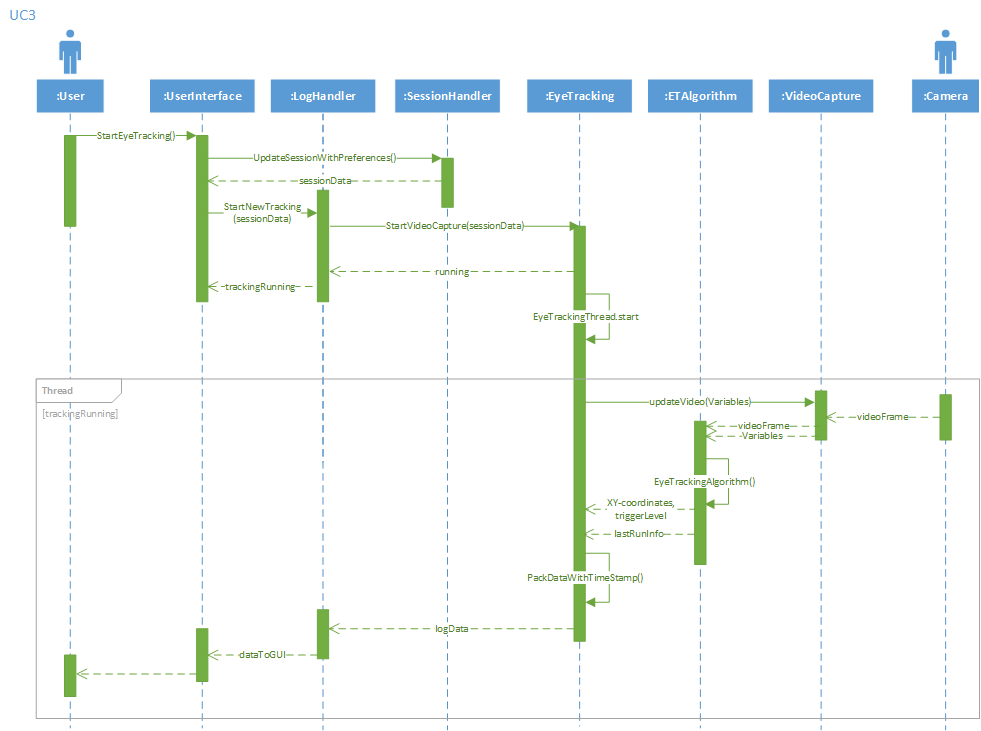
\includegraphics[width=1\linewidth]{UC3}
		\caption[Sekvensdiagram - UC3]{Sekvensdiagram for use case 3 - Start måling}
		\label{fig:UC3}
	\end{figure}
	
	Overvejelser om opdelingen af klasser. Hver klasse varetager en opgave med henblik på en af systemets grænseflader. GUI er varetaget af en klasse. De tre genererede filer log, session, og kalibrering er håndteret af tre klasser. Kommunikation med eksternt kamera er håndteret af sin egen klasse. Kommunikation med algoritmen har sin egen klasse. 
		\subsubsection{UserInterface}
		Denne klasse foretager al kommunikation med aktøren \textit{bruger} igennem et grafisk bruger-interface (GUI). For at have en konstant opdatering af interfacet, forventes denne klasse at blive afviklet i egen tråd. 
	
		
		\subsubsection{SessionHandler}
		Her håndteres al data tilknyttet opsætning af eye-tracking-session. 
		\subsubsection{LogHandler}
		Denne klasse håndterer eye-tracking-programmets log-fil. Data fra eye-tracking bliver her pakket og gemt i en log-fil. Kommunikation af målings-relevant data til UserInterface-klassen foretages af denne klasse.
		\subsubsection{VideoCapture}
		Håndtering af data fra kamera eller video-kilde foregår ved hjælp af OpenCV i denne klasse. 
		\subsubsection{EyeTrackingHandler}
	 
		
		\subsubsection{Interaktion mellem klasser}
		
		\begin{figure}
		\centering
		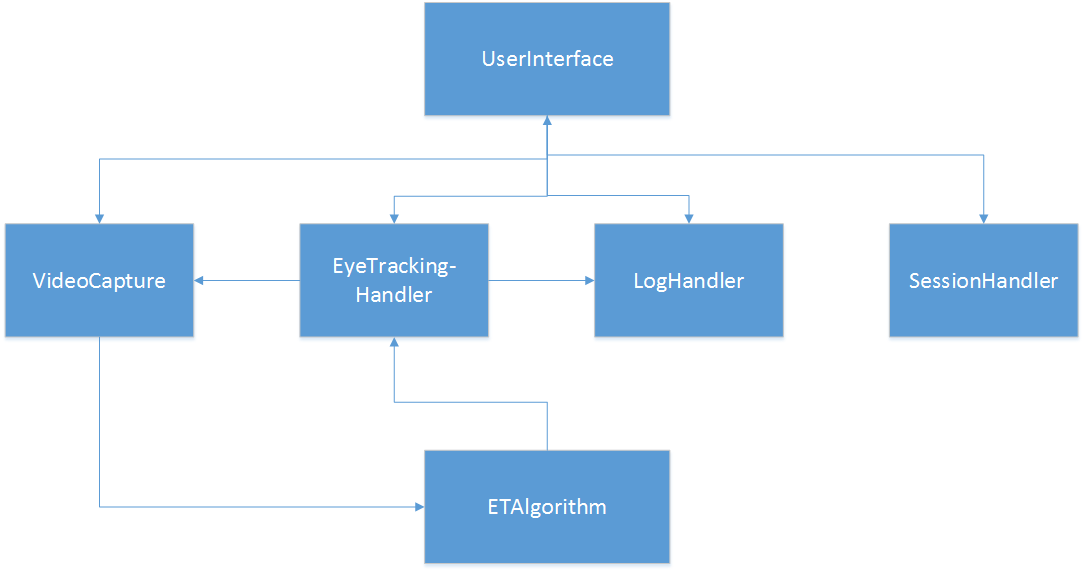
\includegraphics[width=0.9\linewidth]{klasseinteraktion}
		\caption{Klasseinteraktioner}
		\label{fig:klasseinteraktion}
		\end{figure}
	\subsection{Algoritme-arkitektur}
	Klassen ETAlgorithm er kernen af eye-tracking-systemet. Her foretages alle udregninger med henblik på eye-tracking. Denne klasse ønskes isoleret så meget som muligt fra resten af systemet, således at der altid kan foretages ændringer i klassens interne kode, uden at det påvirker resten af systemet. Konsistente grænseflader for denne klasse er derfor essentielt. 
	ETAlgorithm bliver håndteret af klassen EyeTracking, modtager et videosignal og et sæt af variabler, og returnerer XY-koordinat, trigger-niveau, samt et sæt af variabler. 
	
	Da program API'en skal kunne understøtte forskellige typer af eye-tracking-algoritmer, har det været nødvendigt at definere inputs og outputs for algoritmeklasse ETAlgorithm. Input-strukturen består af en video-frame i korrekt format givet af OpenCV-arkitekturen, kalibreringsdata, og et sæt af 16 frie variabler. Disse variabler har på forhånd ikke noget format, og giver derfor brugeren mulighed for at videregive en række værdier til algoritmen uanset format. Herved kan enhver algoritme med op til 10 inputvariabler implementeres uden nødvendighed for ændringer i API'en.\\
	\\
	 For eksempel benytter dette projekt sig af en række variabler til at angive: koordinater for sidste pupil-center, afgrænsninger af sidste sæt øjne, hvorvidt Viola Jones skal køres, thresholdværdier, og maks antal RANSAC-iterationer.  Disse værdier indeholder både arrays, matricer, enkelt værdier og  booleans.
	\\
	De 10 frie inputvariablers startværdier kan indstilles fra GUI, og gemmes i præference-filen. 
	\subsection{Bruger-interface}
	Interfacet er designet med henblik på intuitivt brug, så ledes at det ikke er nødvendigt med dybere introduktion til programmet. Forskellige stadier af hvad man kan gøre i interfacet reducerer muligheden for uønskede handlinger. Det er for eksempel ikke muligt at starte eye-tracking før nødvendig opsætning er fuldført. 
	
	Figur \ref{fig:FrameworkUdkastSimpel} beskriver det forventede grafiske bruger interface. Interfaces er designet ud fra use case diagrammerne beskrevet i kravspecifikationen.
	De fire faner til højre i interfacet - notes, video, calibration, algorithm - tillader brugeren at læse og inputte ønskede præferencer. Følgende værdier er tilstede:
	\begin{itemize}
		\item Notes: Noter til bruger af systemet. Disse har ingen funktion for programmet.
		\item Screen 2 resolution: Angiver opløsningen på skærmen brugt i opstillingen (se figur \ref{???}). Opløsningen angives som bredde og højde adskilt af 'x'.
		\item Log filename: Alternativt navn for log-filen. Er feltet tomt bliver der auto-genereret et navn af formatet YYMMDD-HHMM (år måned dato - time minut). 
		\item Session path: Peger på fil-stien hvor sessionsfilerne (præferencer, log og kalibrering) bliver oprettet. Bliver selv skrevet ind af programmet når  man opretter en ny session. 
		\item Using camera source?: Angiver hvorvidt der bliver brugt kamera eller video-fil som input til algoritmen. 
		\item Source: Hvis der er valgt kamera, peget denne værdi på kamera-kilden. Hvis der er valgt video-fil, fortæller denne filstien. 
		\item Recording video?: Angiver hvorvidt det brugte input skal gemmes som en ny video-fil. 
		\item Filepath for recorded data: Angiver hvor den generede video-fil skal gemmes. Hvis intet er angivet gemmes filen i session path. 
		\item Calibration type: Beskriver hvilken type kalibrering der skal benyttes. Man kan således have flere forskellige kalibreringstyper. 
		\item Load calibration file: Giver mulighed for at vælge en allerede oprette kalibreringsfil. Når en ny kalibrering er fuldført, vil denne værdi pege på den nye fil.
		\item New calibration log filename: Angiver navnet på den oprettede kalibreringsfil. Hvis intet er angivet gemmes filen i session path med navnet calibration.clog. 
		\item V1 til V10: Angiver ti frie variabler til brug i algoritmen. Felterne name bliver ikke benyttet af systemet, og er blot til brugerens nytte. Felterne value kan indeholde alt der opfylder korrekt syntaks for Python og Numpy-biblioteket. 
	\end{itemize}		
	\begin{figure}
		\centering
		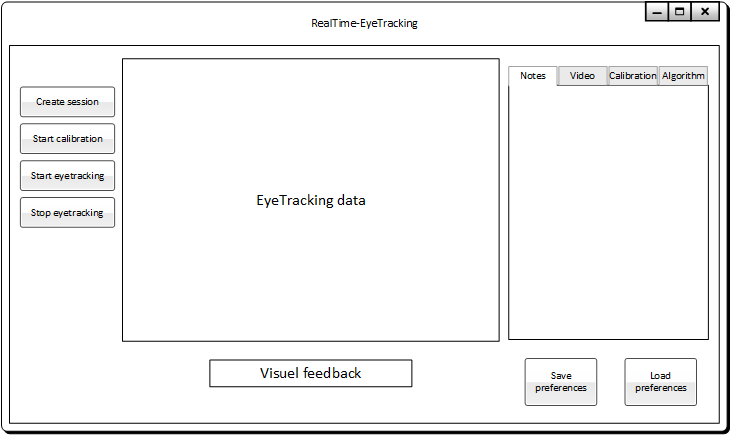
\includegraphics[width=0.9\linewidth]{FrameworkUdkastSimpel}
		\caption[Udkast til GUI]{Udkast til det grafiske bruger-interface}
		\label{fig:FrameworkUdkastSimpel}
	\end{figure}
	
	
	
	\subsection{Diskussion}
\end{document}